\section{IP}
IP is the protocol that binds the various elements in the transport
layer together. When a packet is send from the transport layer (with
TCP/UDP), it is wrapped in an IP datagram. It is this datagram that is
sent to the network layer. We will give a short explanation on IPv4
and IPv6 below.

\subsection{IPv4}
IPv4 is currently the protocol that is in use. The format of an IPv4
datagram can be seen below:

\begin{figure}
  \begin{center}
    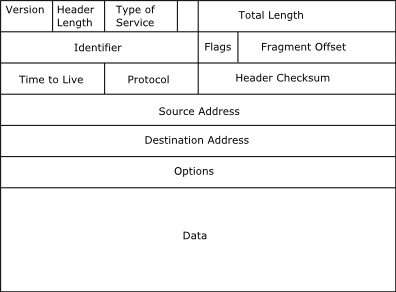
\includegraphics[scale=0.5]{IPv4dg.png}
  \end{center}
\end{figure}

The IP datagram header is 20 bytes, if it carries a TCP datagram, the
size is 40 bytes (in headers).

An IPv4 address consists of 32-bits, and is separted by dots with 8
bits in each space. It is viewed with its decimal representation of
the bits.

The subnet addresses of a network are usually defined with the CIDR
(pronouced cider) notation. The address is written as normal with
x.x.x.x, but with a slash in the end and the number of bits that
define the subnet address. So x.x.x.x/24, as an example.

\subsection{IPv6}
IPv6 is supposed to be the successor of IPv4. The format of an IPv6
datagram can be seen below:

\begin{figure}
  \begin{center}
    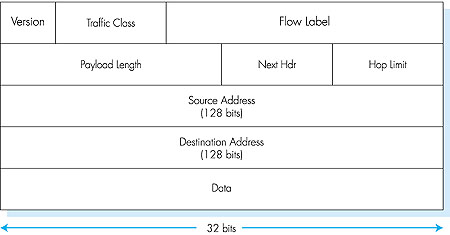
\includegraphics[scale=0.5]{04-40.jpg}
  \end{center}
\end{figure}

The biggest difference is that IPv6 does not allow
fragmentation. Furthermore there is no header checksum, since the
protocols in the transport layer and link layer already check the
sums.

\subsection{IPv4 vs IPv6}

\subsection{Fragmentation}
Not all link-layer protocols can carry the same amount of data. To
make up for this, an IP datagram can be broken into smaller chunks so
the packet can be delivered. The maximum size of a packet that can be
transmitted is called \textbf{maximum transmission unit} or MTU.

IP keeps track of the packets with the \textit{identification},
\textit{flag}, and \textit{fragmentation offset} fields seen in the
format the datagram.

Note that IPv6 does not allow fragmentation. Instead it encourages
packets to be split, before being sent.